%% ID: spouting_can
%% TITLE: The Spouting Can
%% TYPE: question
%% QUESTIONTYPE: symbolic
%% CONCEPTS: energy, eq_of_motion_diff
%% VIDEOS: 
%% LEVEL: 4
%% TOPIC: mechanics/dynamics
%% ORDER: 10

\begin{problem}[IntA1983PIQ16l] 
{The 'spouting can', as shown in Figure \ref{fig:Dynamics_Spouting_Can}, is sometimes used to demonstrate the variation of pressure with depth. When the corks are removed from the tubes in the side of the can, water of density \vari{\rho} flows out with a speed that depends on depth.

\begin{figure}[h]
	\centering
	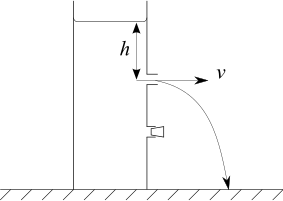
\includegraphics[width=0.4\textwidth]{../../../figures/Dynamics_Spouting_Can.svg}
	\caption{}\label{fig:Dynamics_Spouting_Can}
\end{figure}

\begin{enumerate} 
\item If the level of water in the can is maintained constant, calculate the work done by hydrostatic pressure when volume \vari{\Delta V} leaves a tube at a depth \vari{h} below the surface. 

\item Assuming that all this work provides the kinetic energy of the emerging water, show that the speed \vari{v} of efflux (outflow) is \vari{\sqrt{2gh}}.

\item In a certain can, the three tubes are set at equal distances \vari{a} above the base of the can. When asked to draw the paths of the water coming from the three jets (the overall depth of the water being \vari{4a}), a student made the sketch shown  in Figure \ref{fig:Dynamics_Spouting_Can_2}. Find the values of the distances \vari{x_{1}}, \vari{x_{2}} and \vari{x_{3}} in terms of \vari{a}, and sketch a better diagram. \end{enumerate}

\begin{figure}[h]
	\centering
	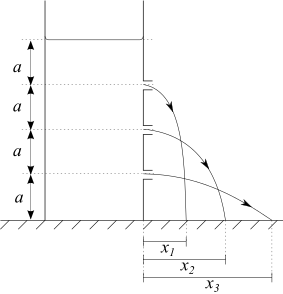
\includegraphics[width=0.4\textwidth]{../../../figures/Dynamics_Spouting_Can_2.svg}
	\caption{}\label{fig:Dynamics_Spouting_Can_2}
\end{figure}
}{
\stress{Used with permission from UCLES, A Level Physics, November 1983, Paper 1, Question 16}
}{\begin{enumerate}
\item The key equation is \valuedef{P}{h\rho g}{}, where \vari{P} is pressure \valuedef{}{\frac{\text{force, F}}{\text{area, A}}}{}. With some rearranging we can get this into a more useful form for the information we have been given:

\begin{eqnarray*} 
\left(\frac{F}{A}\right) &= h \rho g\\ 
F&= h \rho g A  
\end{eqnarray*}
Hence work done, \vari{W}, is 
\begin{eqnarray*}
W &=  F\Delta d \\
&= h \rho g A\Delta d\\
&=h\rho g\Delta V 
\end{eqnarray*}


\item Use conservation of energy, equating work done (just calculated) to kinetic energy

\begin{equation*}
 \frac{1}{2}mv^{2} = h \rho g \Delta V
\end{equation*} 
And, since \valuedef{\Delta V \times \rho}{}{mass,}\vari{m} 
\begin{equation*} 
 & \frac{1}{2}mv^{2} = mgh 
 \end{equation*}

(Where, in both cases, \vari{m} is the mass of the water flowing out through the hole). Hence solve for speed, \vari{v}:

\begin{eqnarray*}
& v^{2} = 2gh \\
& v = \sqrt{2gh}
\end{eqnarray*}


\item We are interested in how far the water travels horizontally, which we can find using \valuedef{distance}{speed \times time}{}. However, since each hole is at a different height (hence also a different depth below the surface), both the horizontal speed and the time taken for the water to fall to the ground will be different for the holes. We will have to create a general equation for \vari{x_{n}}, where \valuedef{n}{1}{} represents the top hole, \valuedef{n}{2}{} the middle hole and \valuedef{n}{3}{} the bottom hole. It is easy to find an expression for the speed out of each hole \vari{v_{n}} using the equation calculated above: \valuedef{h}{na}{}, so \valuedef{v_{n}}{\sqrt{2gna}}{}. Now we can use SUVAT to find an expression for \vari{t_{n}}.

Vertically:
\begin{eqnarray*}
 s&= ut + \frac{1}{2}at^{2}
\end{eqnarray*} 
The height above ground is given by \vari{\left(4-n\right)a}:
\begin{eqnarray*}
\left(4-n\right)a&= \frac{1}{2}gt_{n}^{2} \\ 
\Rightarrow t_{n}&= \sqrt{\frac{2a\left(4-n\right)}{g}}
\end{eqnarray*}

Now horizontally:
\begin{eqnarray*} 
x_{n}&= v_{n}t_{n}
\end{eqnarray*}  
Substituting in our expressions for \vari{v_{n}} and \vari{t_{n}}:
\begin{eqnarray*}
 x_{n}&= \sqrt{2gna}\times\sqrt{\frac{2a\left(4-n\right)}{g}} \\ 
\Rightarrow x_{n}&= \sqrt{4na^2\left(4-n\right)} \\ 
\end{eqnarray*}

Putting in \valuedef{n}{1}{}, 2 and 3 we find that

\begin{equation*}
x_1 = 2\sqrt{3}ga \quad\quad\quad\quad x_2 = 4ga \quad\quad\quad\quad x_3 = 2\sqrt{3}ga
\end{equation*}

So the sketch will look a little different to the one given in the question, with the water from hole \vari{2} travelling the furthest. A better sketch is presented in Figure \ref{fig:Dynamics_Spouting_Can_3}.

\begin{figure}[h]
	\centering
	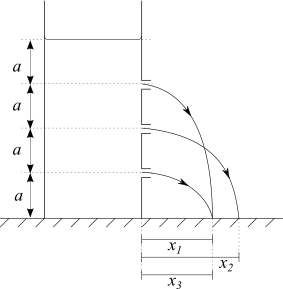
\includegraphics[width=0.4\textwidth]{../../../figures/Dynamics_Spouting_Can_3.svg}
	\caption{}\label{fig:Dynamics_Spouting_Can_3}
\end{figure}

\end{enumerate}
}
\end{problem}